% Options for packages loaded elsewhere
\PassOptionsToPackage{unicode}{hyperref}
\PassOptionsToPackage{hyphens}{url}
%
\documentclass[
  english,
  man]{apa6}
\usepackage{lmodern}
\usepackage{amssymb,amsmath}
\usepackage{ifxetex,ifluatex}
\ifnum 0\ifxetex 1\fi\ifluatex 1\fi=0 % if pdftex
  \usepackage[T1]{fontenc}
  \usepackage[utf8]{inputenc}
  \usepackage{textcomp} % provide euro and other symbols
\else % if luatex or xetex
  \usepackage{unicode-math}
  \defaultfontfeatures{Scale=MatchLowercase}
  \defaultfontfeatures[\rmfamily]{Ligatures=TeX,Scale=1}
\fi
% Use upquote if available, for straight quotes in verbatim environments
\IfFileExists{upquote.sty}{\usepackage{upquote}}{}
\IfFileExists{microtype.sty}{% use microtype if available
  \usepackage[]{microtype}
  \UseMicrotypeSet[protrusion]{basicmath} % disable protrusion for tt fonts
}{}
\makeatletter
\@ifundefined{KOMAClassName}{% if non-KOMA class
  \IfFileExists{parskip.sty}{%
    \usepackage{parskip}
  }{% else
    \setlength{\parindent}{0pt}
    \setlength{\parskip}{6pt plus 2pt minus 1pt}}
}{% if KOMA class
  \KOMAoptions{parskip=half}}
\makeatother
\usepackage{xcolor}
\IfFileExists{xurl.sty}{\usepackage{xurl}}{} % add URL line breaks if available
\IfFileExists{bookmark.sty}{\usepackage{bookmark}}{\usepackage{hyperref}}
\hypersetup{
  pdftitle={School Socioeconomic Status Context and Social Skills in Children},
  pdfauthor={Philip Parker1, Taren Sanders1, Jake Anders2, Nikki Shure2, John Jerrim2, Michael Noetel1,3, \& Joseph Ciarrochi1},
  pdflang={en-EN},
  pdfkeywords={social skills; assimilation effects; socioeconomic status; school context},
  hidelinks,
  pdfcreator={LaTeX via pandoc}}
\urlstyle{same} % disable monospaced font for URLs
\usepackage{graphicx}
\makeatletter
\def\maxwidth{\ifdim\Gin@nat@width>\linewidth\linewidth\else\Gin@nat@width\fi}
\def\maxheight{\ifdim\Gin@nat@height>\textheight\textheight\else\Gin@nat@height\fi}
\makeatother
% Scale images if necessary, so that they will not overflow the page
% margins by default, and it is still possible to overwrite the defaults
% using explicit options in \includegraphics[width, height, ...]{}
\setkeys{Gin}{width=\maxwidth,height=\maxheight,keepaspectratio}
% Set default figure placement to htbp
\makeatletter
\def\fps@figure{htbp}
\makeatother
\setlength{\emergencystretch}{3em} % prevent overfull lines
\providecommand{\tightlist}{%
  \setlength{\itemsep}{0pt}\setlength{\parskip}{0pt}}
\setcounter{secnumdepth}{-\maxdimen} % remove section numbering
% Make \paragraph and \subparagraph free-standing
\ifx\paragraph\undefined\else
  \let\oldparagraph\paragraph
  \renewcommand{\paragraph}[1]{\oldparagraph{#1}\mbox{}}
\fi
\ifx\subparagraph\undefined\else
  \let\oldsubparagraph\subparagraph
  \renewcommand{\subparagraph}[1]{\oldsubparagraph{#1}\mbox{}}
\fi
% Manuscript styling
\usepackage{upgreek}
\captionsetup{font=singlespacing,justification=justified}

% Table formatting
\usepackage{longtable}
\usepackage{lscape}
% \usepackage[counterclockwise]{rotating}   % Landscape page setup for large tables
\usepackage{multirow}		% Table styling
\usepackage{tabularx}		% Control Column width
\usepackage[flushleft]{threeparttable}	% Allows for three part tables with a specified notes section
\usepackage{threeparttablex}            % Lets threeparttable work with longtable

% Create new environments so endfloat can handle them
% \newenvironment{ltable}
%   {\begin{landscape}\begin{center}\begin{threeparttable}}
%   {\end{threeparttable}\end{center}\end{landscape}}
\newenvironment{lltable}{\begin{landscape}\begin{center}\begin{ThreePartTable}}{\end{ThreePartTable}\end{center}\end{landscape}}

% Enables adjusting longtable caption width to table width
% Solution found at http://golatex.de/longtable-mit-caption-so-breit-wie-die-tabelle-t15767.html
\makeatletter
\newcommand\LastLTentrywidth{1em}
\newlength\longtablewidth
\setlength{\longtablewidth}{1in}
\newcommand{\getlongtablewidth}{\begingroup \ifcsname LT@\roman{LT@tables}\endcsname \global\longtablewidth=0pt \renewcommand{\LT@entry}[2]{\global\advance\longtablewidth by ##2\relax\gdef\LastLTentrywidth{##2}}\@nameuse{LT@\roman{LT@tables}} \fi \endgroup}

% \setlength{\parindent}{0.5in}
% \setlength{\parskip}{0pt plus 0pt minus 0pt}

% \usepackage{etoolbox}
\makeatletter
\patchcmd{\HyOrg@maketitle}
  {\section{\normalfont\normalsize\abstractname}}
  {\section*{\normalfont\normalsize\abstractname}}
  {}{\typeout{Failed to patch abstract.}}
\patchcmd{\HyOrg@maketitle}
  {\section{\protect\normalfont{\@title}}}
  {\section*{\protect\normalfont{\@title}}}
  {}{\typeout{Failed to patch title.}}
\makeatother
\shorttitle{School SES and Social Skills}
\keywords{social skills; assimilation effects; socioeconomic status; school context\newline\indent Word count: X}
\DeclareDelayedFloatFlavor{ThreePartTable}{table}
\DeclareDelayedFloatFlavor{lltable}{table}
\DeclareDelayedFloatFlavor*{longtable}{table}
\makeatletter
\renewcommand{\efloat@iwrite}[1]{\immediate\expandafter\protected@write\csname efloat@post#1\endcsname{}}
\makeatother
\usepackage{lineno}

\linenumbers
\usepackage{csquotes}
\ifxetex
  % Load polyglossia as late as possible: uses bidi with RTL langages (e.g. Hebrew, Arabic)
  \usepackage{polyglossia}
  \setmainlanguage[]{english}
\else
  \usepackage[shorthands=off,main=english]{babel}
\fi
\newlength{\cslhangindent}
\setlength{\cslhangindent}{1.5em}
\newenvironment{cslreferences}%
  {\setlength{\parindent}{0pt}%
  \everypar{\setlength{\hangindent}{\cslhangindent}}\ignorespaces}%
  {\par}

\title{School Socioeconomic Status Context and Social Skills in Children}
\author{Philip Parker\textsuperscript{1}, Taren Sanders\textsuperscript{1}, Jake Anders\textsuperscript{2}, Nikki Shure\textsuperscript{2}, John Jerrim\textsuperscript{2}, Michael Noetel\textsuperscript{1,3}, \& Joseph Ciarrochi\textsuperscript{1}}
\date{}


\authornote{

The authors made the following contributions. Philip Parker: Conceptualization, Formal Analysis, Writing - Original Draft Preparation, Writing - Review \& Editing; Taren Sanders: Conceptualization, Writing - Original Draft Preparation, Writing - Review \& Editing; Jake Anders: Conceptualization, Writing - Original Draft Preparation, Writing - Review \& Editing; Nikki Shure: Conceptualization, Writing - Original Draft Preparation, Writing - Review \& Editing; John Jerrim: Conceptualization, Writing - Original Draft Preparation, Writing - Review \& Editing; Michael Noetel: Conceptualization, Writing - Original Draft Preparation, Writing - Review \& Editing; Joseph Ciarrochi: Conceptualization, Writing - Original Draft Preparation, Writing - Review \& Editing.

Correspondence concerning this article should be addressed to Philip Parker, 33 Berry St, North Sydney, NSW, 2060, Australia. E-mail: \href{mailto:philip.parker@acu.edu.au}{\nolinkurl{philip.parker@acu.edu.au}}

}

\affiliation{\vspace{0.5cm}\textsuperscript{1} Institute for Positive Psychology and Education, Australian Catholic University\\\textsuperscript{2} UCL Institute of Education, UCL\\\textsuperscript{3} School of Health and Behavioural Sciences, Australian Catholic University}

\abstract{
As researchers and policymakers try to understand the consequences of SES for educational and occupational attainment, they increasingly consider social skills to be critical. Yet little research has considered how the school socio-economic context may differentially promote or hinder social skill development. In a representative longitudinal sample of Australian 8-year olds, we tested the association between school average socioeconomic status and social skills as reported by parents and teachers. All models controlled for prior social skills at age 4, and additional school and student covariates. We found that school context was associated with social skill assimilation: controlling for individual socioeconomic status, children in more advantaged schools had more prosocial behavior and fewer peer and conduct problems. We found a consistent interaction between individual and school average socioeconomic status that suggested assimilation effects were only present for children from low socioeconomic backgrounds. We found that children from low socioeconomic backgrounds enter school with lower average social skills. They are more likely to be enrolled in more disadvantaged schools. Finally, the social skills of children from low socioeconomic backgrounds worsen in low SES contexts. Taking the evidence together, social stratified schools may harm children from low SES backgrounds while not benefiting children from high SES backgrounds.
}



\begin{document}
\maketitle

After decades of research and intervention aimed at reducing educational and occupational inequality, inequalities persist (Reardon, 2011). In response to this bleak picture, there has been a flurry of interest in social-emotional competencies driven by the research of Nobel prize-winning economist James Heckman. Heckman (2006) argues that research and intervention on reducing educational inequality have focused too narrowly on ``cognitive'' abilities (generally narrowly deinfed to include ability, IQ, and academic achievement). Yet cognitive abilities are not the only pathway through which low socioeconomic status may stifle educational and occupational attainment. For example, social skills are a potentially powerful explanation for socioeconomic status gaps in educational and occupational attainment (Gutman \& Schoon, 2013). Children from low socioeconomic backgrounds (here after low SES children\footnote{We acknowledge that children themselves do not have a socioeconomic status. Rather they are raised in an environment which is shaped by their parents' socioeconomic status (SES). However, for brevity we refer to children as low SES or high SES hereafter. Likewise, in place of low school average SES and high school average SES we refer to disadvantaged and advantaged schools respectively.}) appear to enter school with poorer social skills (e.g., Jerrim \& Sims, 2019). This is concerning as childhood social skills predict a wide variety of later life outcomes (e.g., Jones, Greenberg, \& Crowley, 2015). Inspired by identity economics, our research asks whether the school context in the stratified school system of Australia may exacerbate this issue. In particular, we explore whether school average socioeconomic status predicts social skills in Year 3 (age 8)---using measures of peer problems, conduct problems, and prosocial behavior. Using prospective representative data, integrated with government administrative data, we found this is that case but that an interaction between student and school SES means that poorer children appear more susceptible to such effects.

\hypertarget{social-skills}{%
\subsection{Social Skills}\label{social-skills}}

Of the skills that employers are looking for when hiring candidates, social skills are some of the most desirable (Rios, Ling, Pugh, Becker, \& Bacall, 2020). Social skills also seem to be a viable target for intervention with meta-analysis showing social and emotional learning programs have moderate effects on improving key social skills like reducing conduct problems and improving social-emotional learning skills and prosocial behavior (Durlak, Weissberg, Dymnicki, Taylor, \& Schellinger, 2011). Social skills appear to be worthwhile targets from a societal perspective given their relationship to academic achievement (Corcoran, Cheung, Kim, \& Xie, 2018) and their role in predicting adult employment, crime, public assistance, substance abuse, and mental health (Jones et al., 2015). Among young children, it is increasingly common to focus on social skills as measured by the Strengths and Difficulties Questionnaire (see Datta Gupta \& Simonsen, 2010; Gutman \& Schoon, 2013; Jerrim \& Sims, 2019). We use this questionnaire to measure peer problems, conduct problems, and prosocial behavior. We model social skills using both parent and teacher reports. Measures of SES at the student level are taken from in-person interviews with parents and school SES (as well as student achievement) is taken from government administrative records.

\hypertarget{contrast-processes-and-identity-economics}{%
\subsection{Contrast Processes and Identity Economics}\label{contrast-processes-and-identity-economics}}

Children's social skills depend in part on the context in which they develop (Jerrim \& Sims, 2019). There are two major forces in social psychology---assimilation and contrast (Mussweiler, Rüter, \& Epstude, 2004)---that may account for how school context affects children's social skill development. Contrast processes are in operation when children's perceptions, opinions, or behavior depend on their perceived rank order within their group. Assimilation processes are in operation when people's perceptions, opinions, or behaviour depend on reference group norms (Kelley, 1952).

The theory of \emph{Identity Economics} implies an assimilative effect (Akerlof \& Kranton, 2010). Identity Economics argues that the social context of the school possesses a gravity that attracts students' identity, values, and behavior toward the prototypical identity, values, and behavior of the school (Akerlof \& Kranton, 2002). School ethos and norms around behavior incentivize children to act in a manner consistent with these norms. School average socioeconomic status could, thus, affect social skills. A now large body of research shows that social skills are correlated with socioeconomic status (SES; de Laat, Essink-Bot, van Wassenaer-Leemhuis, \& Vrijkotte, 2016; Garratt, Chandola, Purdam, \& Wood, 2017; McMunn, Nazroo, Marmot, Boreham, \& Goodman, 2001; Rajmil et al., 2014) and, this relationship is present before children enter school (Washbrook \& Waldfogel, 2011). In socially stratified school systems, children of similar SES tend to be schooled together. Thus, if children assimilate to the school context they are in, as Identity Economics would suggest, we would expect school average socioeconomic status to influence the development of social skills.

Jerrim and colleagues (2019) provide one test of the potential assimilative effect of schools on social skills. They found that living in an area with selective schools is associated with better social skills when compared to children living in districts without a selective school. They also found some assimilative effects of school average SES predicting social skills using the total score of the strengths and difficulties questionnaire (SDQ). The assimilation effects they found, however, were weak. This may be because the authors used the SDQ total score---which includes a range of social and emotional behaviors---rather than focusing on specific social skill components of the SDQ. Further, assimilative effects may be non-linear. Put another way, the assimilative power of school contexts may not be evenly distributed across the socioeconomic distribution. This is an important consideration that research has not hitherto considered, though differential assimilation across the socioeconomic status gradient has been theorized (Gradstein \& Justman, 2005).

\hypertarget{current-study}{%
\section{Current Study}\label{current-study}}

Australia is the context of our research. Australia is a useful country to focus on because Australia's Programme for International Student Assessment (PISA) Index of Social Inclusion score is relatively low (OECD, 2015). This means that Australian schools are socially stratified (Parker, Guo, \& Sanders, 2019; Parker et al., 2018). Our major hypothesis is that school average socioeconomic status will have an assimilation effect on association with social skills at Year 3 (age 8) controlling for incoming social skills (age 4), individual socioeconomic status (age 4) and a range of demographic and achievement covariates\footnote{This assimilation effect will be indicated by a negative coefficient for peer problems and conduct problems regressed on school average socioeconomic status and a positive coefficient for prosocial behavior regressed on school average socioeconomic status. This is because of the way in which these factors are valanced (high scores indicate high levels of prosocial behavior, but also high levels of peer and conduct problems).}. We also anticipate that there will be differential associations of school average socioeconomic status on social skills across the socioeconomic status gradient.

We expect the assimilation effects to occur in the context of low SES children entering school with poorer social skills (de Laat et al., 2016; Garratt et al., 2017; McMunn et al., 2001; Rajmil et al., 2014). Given Australian schools are socially stratified (OECD, 2015; Parker et al., 2018), we expect low SES children to attend more disadvantaged schools on average.

\hypertarget{method}{%
\section{Method}\label{method}}

\hypertarget{participants-and-study-design}{%
\subsection{Participants and Study Design}\label{participants-and-study-design}}

\begin{figure}
\centering
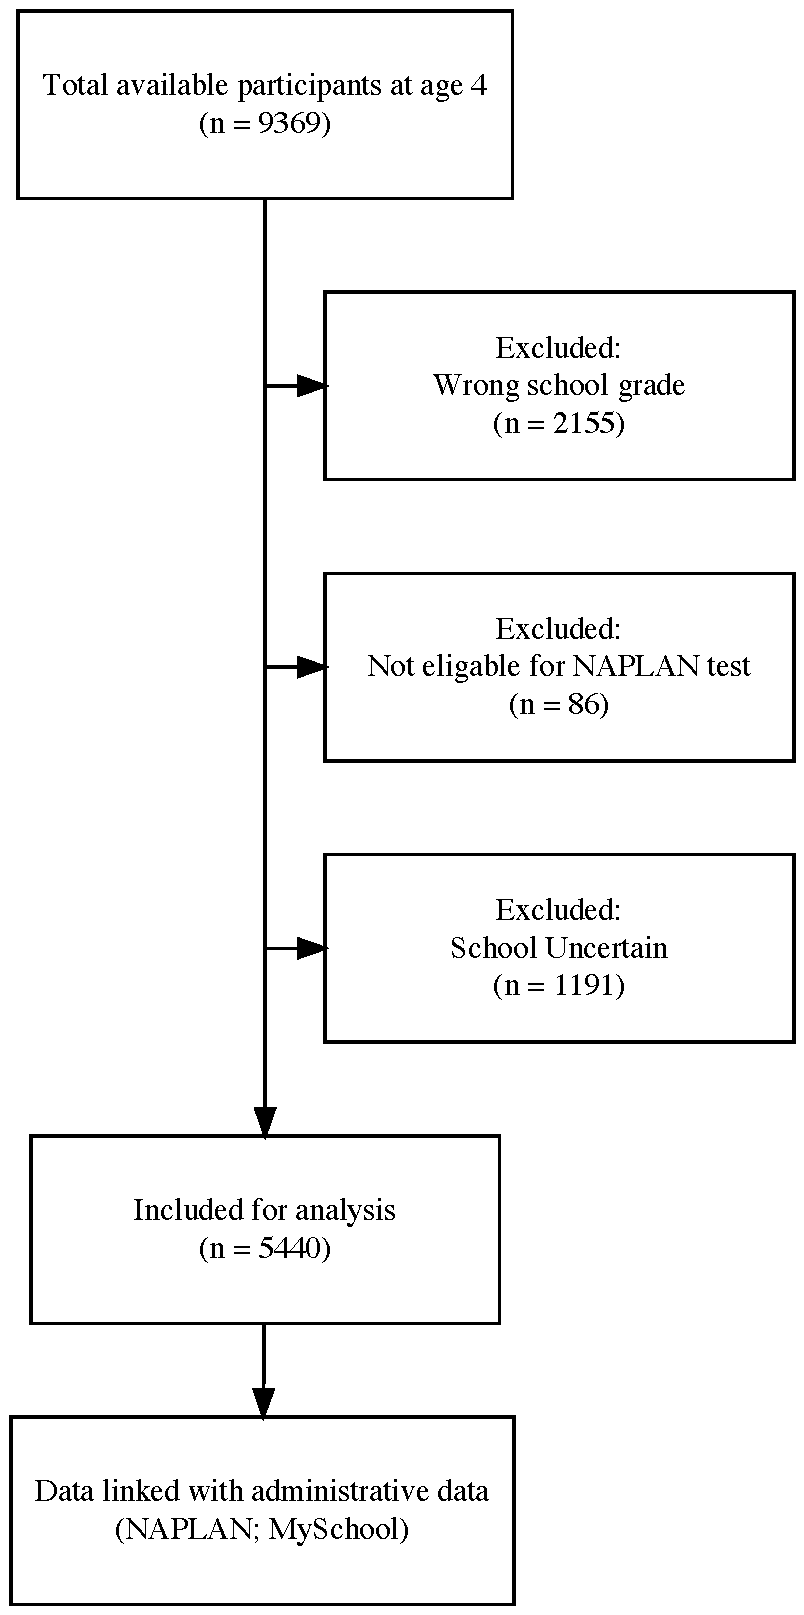
\includegraphics{/Users/tasanders/GitHub/social_skills_2020/fig/flow.pdf}
\caption{\label{fig:consort}Participant flow diagramme}
\end{figure}

We use data for children, their parents, and their teachers from the B-Cohort and K-Cohort of the Longitudinal Study of Australian Children (LSAC). LSAC is a government-run study of a representative sample of Australian children who were zero-one (B-cohort) or four-five (K-Cohort) years of age in 2004. Both cohorts of children have been followed every two years since (AIFS, 2015). LSAC includes linked administration records for student performance in a standardized national numeracy test. We also use government collected data on school average socioeconomic status. Many children in the sample were the only child surveyed (25.75\%) or were one of two children surveyed (20.96\%) in their school. By using administrative records, we gain school average socioeconomic status based on the child's \(\text{\underline{whole}}\) school grade from a high-quality source, thus avoiding sampling bias present in much school context research. We excluded participants who were not in school (e.g., were home schooled, or were otherwise missing an identifier of which school they attended), were not in Year 3 at the time of testing, or were not eligible to complete national standardized testing (e.g., children with an intellectual disability). Together our total sample was 5440 (52.08\% boys) children in Year 3 at school (\textasciitilde age 8). In the vast majority of cases (98\% ), parent data came from mothers. A participant flow diagram is presented in Figure \ref{fig:consort} including the number of participants excluded because there were a) not in Year 3 during the age 8 LSAC data collection sweep; b) were not eligible to participate NAPLAN (e.g., due to intellectual disability; or c) were not enrolled in school (e.g., were home schooled).

\hypertarget{measures}{%
\subsection{Measures}\label{measures}}

\hypertarget{social-skills-at-age-4-and-8}{%
\subsubsection{Social skills at age 4 and 8}\label{social-skills-at-age-4-and-8}}

Social skills were estimated using the peer problems, conduct problems, and prosocial behavior component scores from the SDQ (Goodman, 1997). We explored social skills at age 4-5 (for prior social skills; parent report only) and age 8-9 (as primary outcomes) as reported by the child's \emph{parent} and the child's \emph{teacher}. The SDQ asks respondents to rate a child's behavior in the last six months on a 3-point scale (not true, somewhat true, and certainly true). Questions ask about the child's peer problems (``Rather solitary, tends to play alone''), conduct problems (``Often fights with other children or bullies them''), and prosociality (``Is kind to younger children''). Greatest lower bound estimates of reliability were all greater than .95 and parallel analysis suggested that a single component was sufficient for each of the parent and teacher and age 4 and age 8 social skills factors. On the basis of this evidence, we used the total scores for these scales as developed by the LSAC administrators. Scores ranged from 0 to 10. These scores were heavily left censored for peer and conduct problems with a preponderance of students being scored as a zero by their parent or teacher. Prosocial behaviors were heavily right censored. Censoring can be viewed as a special type of missing data where scores on \(y*\) (the hypothesised true latent distribution of the variable) below or above the bounds are curtailed to fit within the bounds resulting in the observed scores \(y\) (Gelman, Hill, \& Vehtari, 2020). Models accounting for this censoring were used in all cases with results provided on the scale of the latent variable \(y*\) believed to underlie the censored variable (hence negative predicted scores or scores over 10 were possible).

Parents and teachers had moderate agreement for children at age 8 with correlations ranging from \emph{r} = 0.41 95\% CI{[}0.38, 0.43{]} for peer and \emph{r} = 0.39 95\% CI{[}0.37, 0.42{]} for conduct problems to \emph{r} = 0.29 95\% CI{[}0.26, 0.31{]} for prosocial behavior.

\hypertarget{socioeconomic-status}{%
\subsubsection{Socioeconomic Status}\label{socioeconomic-status}}

\emph{Individual SES} was measured using the Socioeconomic Position (SEP) index constructed by the LSAC survey organizers (Baker, Sipthorp, \& Edwards, 2017). The SEP index is constructed from parent reported standardized weekly income, years of education, and ANU4 occupational prestige derived from the Australian Standard Classification of Occupations. The SEP has a mean of zero and a standard deviation of one.

\emph{School average SES} was measured using the Index of Community Socioeconomic Advantage (ICSEA) that the Australian government uses to assess the relative advantage of schools for the purpose of funding allocation and policy. This measure was taken from government administration records. ICSEA has a mean of 1000 and a standard deviation of 100. We z-scored this variable for analysis.

\hypertarget{covariates}{%
\subsubsection{Covariates}\label{covariates}}

Numeracy for the child and for their complete school grade was taken from administration records of National Assessment Program -- Literacy and Numeracy (NAPLAN) test results. The relevant NAPLAN tests for this study are given to all eligible children in the country in Year 3 (age 8). The tests are scaled so they are comparable across age cohort and across year grade. These high-stakes tests have a mean of 500 and a standard deviation of 100. Included in the analysis was the first principal component of the numeracy, grammar, spelling, reading, and writing scores from NAPLAN\footnote{Parallel analysis suggested a single principal component was sufficient to account for the variation in the NAPLAN scores.}. For verbal ability (as a proxy for cognitive school readiness) we used the Peabody Picture Vocabulary test (Dunn \& Dunn, 2007) given to participants at age 4 (i.e., at or just before school commencement). Cohort was included as a covariate in all models as was measures of rural status and gender---all measured at age 4. The sector (government or non-government) of the school the child attended was also included as a covariate.

\hypertarget{analysis}{%
\subsection{Analysis}\label{analysis}}

There was a relatively small amount of missing data for most variables. However, given the data were longitudinal and included both linked administrative records and data collected from both the child's teacher and parent, missing data was inevitable. Attrition was offset by applying combined sample and attrition weights constructed for the age 8 sample. Remaining missing data was small with the largest missing data proportion for teacher reported social skills at 14\%. All other variables had 6\% missing data or less (see code book in supplementary materials ). To account for this, we constructed five imputed datasets using a bootstrapped expectation maximization procedure from the Amelia II package (Honaker, King, \& Blackwell, 2011). These imputations were used in all analyses. All analyses were done using Bayes via the BRMS package in R (Bürkner, 2017). The Bayes models were run once for each imputation and then the resulting posterior samples were pooled before estimates and their uncertainty were extracted. Interactions and their associated uncertainties were plotted by taking marginal effect estimates from a random 500 posterior draws for disadvantaged (two standard deviations below the mean of SES), average, and advantaged (two standard deviations above the mean of SES) students (Gelman et al., 2020).

All models in the paper that predicted social skills were estimated taking into account the censoring of the social skills means using a Bayes version of Tobit regression. Tobit models can be used when seeking to model outcome variables that are censored on the left, right, or both tails (see Kleiber \& Zeileis, 2008). As scores on the social skills variables have both a floor of zero and a ceiling of 10, we included censoring on both the left and the right in all models. The multilevel nature of the data (children nested within schools) was addressed by the inclusion of a random intercept for schools. We clearly demarcate the units of analysis in tables and figures. In general the SDQ measures are retained on the original scale and all other continuous variables are z-scored. We retain the SDQ scores on the original scale because of the presence of norms (Youth in Mind, 2016). Peer and conduct problems scores of 3 or greater and prosocial scores of 7 or lower place children beyond the `close to average' group and may thus be a potential concern (Youth in Mind, 2016).

The models are fit using the following formula:

\[
\begin{split}
y^{*}_{i} \sim N(\alpha_{j[i]} + X_i\beta, \sigma^{2}_{y}), for~i = 1,...,n \\
\alpha_{j} \sim N(U_j \gamma, \sigma^{2}_{\alpha}), for~j = 1,...k
\end{split}
\]

Here \(X\) is a matrix of individual level predictors for student \(i\) including individual SES, prior social skills, gender, cohort, geographic location, and an NAPLAN achievement index. Prior social skills is particularly critical as this provide stronger conclusions that school context rather than selection effects account for the influence of school average SES on student social skills. Put simply the estimate of school average achievement can be interpreted as the influence of school context on the change in children's social skills from age 4 to age 8. \(U\) is a matrix of school level predictors for school \(j\) including school section and the aforementioned critical variable \emph{school SES}. Note that we predict \(y^{*}_{i}\) which is the latent continuous variable underlying the observed variables which are defined as:

\[
\begin{split}
y_i =  \begin{cases}      
            y*_{i} & \text{if $y*_{i} < 0$ or $y*_{i} > 10 $}\\      
            0 & \text{if $y*_{i} < 0$}\\      
            10 & \text{if $y*_{i} > 10$}    
        \end{cases}
\end{split}
\]

\hypertarget{results}{%
\section{Results}\label{results}}

\hypertarget{low-ses-children-start-school-with-poorer-social-skills-and-enroll-in-more-disadvantaged-schools}{%
\subsection{Low SES Children Start School with Poorer Social Skills and Enroll in More Disadvantaged Schools}\label{low-ses-children-start-school-with-poorer-social-skills-and-enroll-in-more-disadvantaged-schools}}

In order to provide a context for the main analyses we first aimed to show: a) that children from advantaged backgrounds enter school with better social skills (as measured by their parents) and b) that children in Australia tend to be schooled in socially stratified schools. Student SES is slightly correlated with prosocial behaviour (0.05 95\% CI{[}0.023, 0.078{]}) but more strongly and negatively correlated with conduct (-0.18 95\% CI{[}-0.2, -0.15{]}) and peer (-0.16 95\% CI{[}-0.19, -0.13{]}) problems. Children from lower SES backgrounds also tended to enter schools with children from similar backgrounds (0.48 95\% CI{[}0.46, 0.51{]}).

\captionsetup[table]{labelformat=empty,skip=1pt}
\begin{longtable}{llrrr}
\caption*{
\large Table 1\\ 
\small Effect of School Average SES on Social Skills\\ 
} \\ 
\toprule
Outcome & Report Source & Estimate & -95\% CI & +95\% CI \\ 
\midrule
conduct & teacher & $-0.154$ & $-0.264$ & $-0.043$ \\ 
social & teacher & $0.148$ & $0.054$ & $0.242$ \\ 
peer & teacher & $-0.116$ & $-0.204$ & $-0.029$ \\ 
conduct & parent & $-0.108$ & $-0.170$ & $-0.046$ \\ 
social & parent & $0.087$ & $0.018$ & $0.155$ \\ 
peer & parent & $-0.134$ & $-0.203$ & $-0.063$ \\ 
\bottomrule
\end{longtable}

\hypertarget{school-average-ses-predicts-social-skills-controlling-for-age-4-ses-and-social-skills}{%
\subsection{School Average SES Predicts Social Skills Controlling for Age 4 SES and Social Skills}\label{school-average-ses-predicts-social-skills-controlling-for-age-4-ses-and-social-skills}}

We next predicted social skills with school average SES controlling for individual SES, a range of demographic covariates and academic performance measures, and social skills at age 4. Results for school average SES are presented under in Table \ref{tab:table-1} (the full model results are in supplementary materials). Because we control for prior social skills, the effects of school average SES in these models can be interpreted as predicting change or development in social skills from age 4 (at or just prior to school enrollment) to age 8 (Year 3). School average SES negatively predicted conduct problems and positively predicted prosocial behavior for both parent and teacher reported social skills. School average SES also negatively predicted peer problems. Results from either teacher or parent provided fairly consistent evidence of the influence of school SES context on social skills (or more specifically change in social skills from age 4 to age 8). Interestingly, the association of school average SES with social skills was similar in strength to the association of individual SES with social skills (see supplementary materials for full results). The effect sizes were equivalent to approximately a 10th of the median absolute deviation in social skills.

\captionsetup[table]{labelformat=empty,skip=1pt}
\begin{longtable}{lllrrr}
\caption*{
\large Table 2\\ 
\small Effect of School Average SES by Student SES on Social Skills\\ 
} \\ 
\toprule
Outcome & Report Source & term & Estimate & -95\% CI & +95\% CI \\ 
\midrule
conduct & teacher & School Average SES & $-0.161$ & $-0.268$ & $-0.054$ \\ 
conduct & teacher & School Average SES by Student SES & $0.150$ & $0.063$ & $0.240$ \\ 
social & teacher & School Average SES & $0.157$ & $0.063$ & $0.250$ \\ 
social & teacher & School Average SES by Student SES & $-0.095$ & $-0.172$ & $-0.020$ \\ 
peer & teacher & School Average SES & $-0.126$ & $-0.218$ & $-0.035$ \\ 
peer & teacher & School Average SES by Student SES & $0.116$ & $0.046$ & $0.189$ \\ 
conduct & parent & School Average SES & $-0.112$ & $-0.176$ & $-0.047$ \\ 
conduct & parent & School Average SES by Student SES & $0.058$ & $0.006$ & $0.110$ \\ 
social & parent & School Average SES & $0.090$ & $0.023$ & $0.157$ \\ 
social & parent & School Average SES by Student SES & $-0.031$ & $-0.087$ & $0.029$ \\ 
peer & parent & School Average SES & $-0.143$ & $-0.213$ & $-0.074$ \\ 
peer & parent & School Average SES by Student SES & $0.117$ & $0.057$ & $0.179$ \\ 
\bottomrule
\end{longtable}

\hypertarget{school-average-ses-predicts-social-skills-mainly-in-low-ses-children}{%
\subsection{School Average SES Predicts Social Skills Mainly in Low SES Children}\label{school-average-ses-predicts-social-skills-mainly-in-low-ses-children}}

The predictive association of school average SES on social skills was not consistent across the SES gradient (see Table \ref{tab:table-2}). Significant school average SES by student SES interactions were significant for peer and conduct problems for both teacher and parent reports and for teacher reported prosocial behavior. Interactions are plotted in Figures \ref{fig:conduct}-\ref{fig:social}. Full model results can be found in supplementary materials. The interaction plots suggest that school context effects were particularly potent for disadvantaged children but school context had minimal impact on social skills for children from advantaged backgrounds. The plots suggest that for the very poorest schools in our sample, the average disadvantaged student would have levels of peer problems greater than the threshold for `close to average' scores and thus potentially of concern (Youth in Mind, 2016). This same child would be well within the `close to average' band in a school with an average levels of SES.

\begin{figure}
\centering
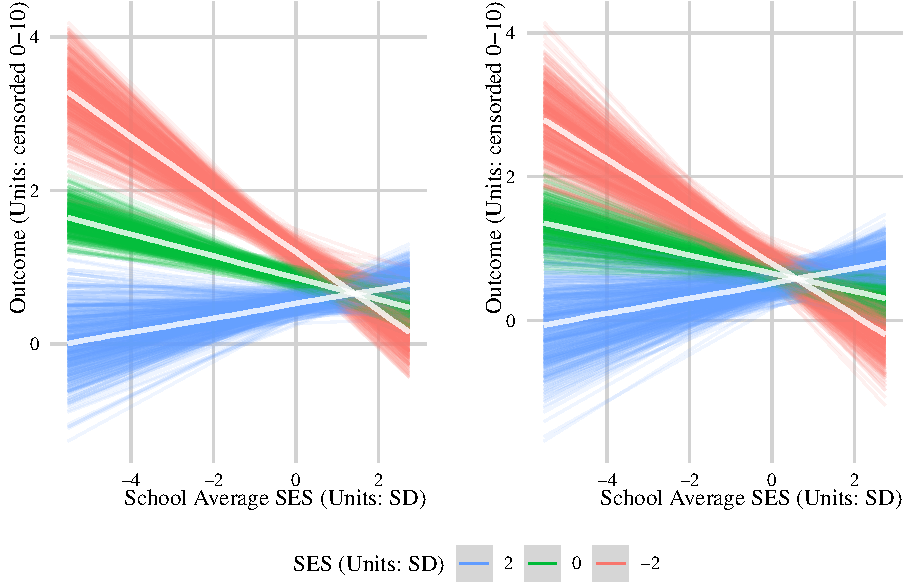
\includegraphics{manuscript_files/figure-latex/peer-1.pdf}
\caption{\label{fig:peer}Interaction Plot for Peer Problems}
\end{figure}

\begin{figure}
\centering
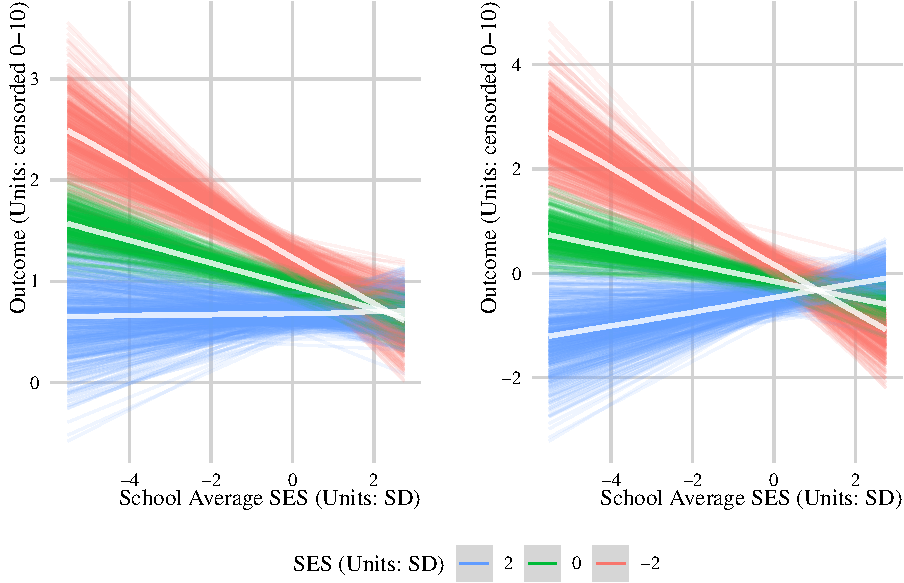
\includegraphics{manuscript_files/figure-latex/conduct-1.pdf}
\caption{\label{fig:conduct}Interaction Plot for Conduct Problems}
\end{figure}

\begin{figure}
\centering
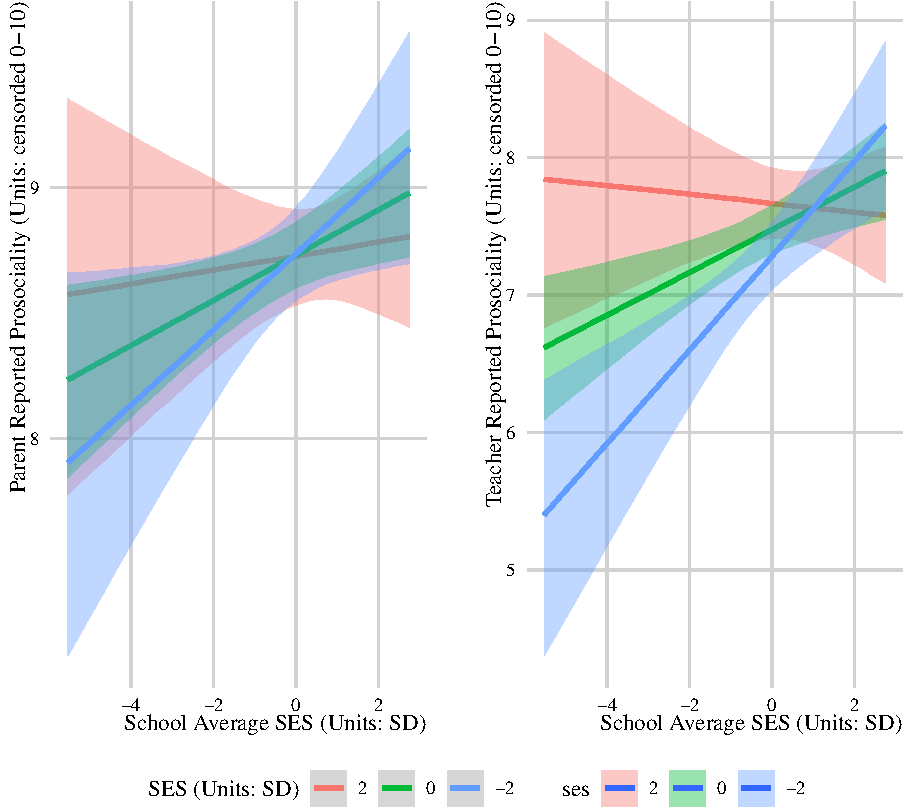
\includegraphics{manuscript_files/figure-latex/social-1.pdf}
\caption{\label{fig:social}Interaction Plot for Prosociality}
\end{figure}

\hypertarget{discussion}{%
\section{Discussion}\label{discussion}}

Research on social skills has repeatedly shown that there is a socioeconomic status gradient to social skills (see Datta Gupta \& Simonsen, 2010; Gutman \& Schoon, 2013; Jerrim \& Sims, 2019). Yet little research in this area has considered the potential influence of school context on social skill development (\emph{cf.} Jerrim \& Sims, 2019). This is a gap that our research sought to fill. Our research considered the association of school socioeconomic context with social skills in early elementary school. We used both parent and teacher reported social skills, finding surprisingly consistent effect sizes regardless of reporting source despite their relatively modest agreement. Importantly, our research used a number of critical controls as well as prior social skills that helped us better identify the effect of school average socioeconomic status. Prior social skills meant that coefficients for school average SES related to change in social skills from age 4 (at or just before school entry) to age 8.

For both teacher and parent reports we found that the association of school context with social skills depended on the individual child's own socioeconomic background. This was the case for all outcomes except for parent reported prosocial behavior. It is worth emphasizing that the nature of these interactions was consistent for all outcomes. Namely, that middle to high SES children were largely unaffected by school socioeconomic context while the children with the lowest socioeconomic status experienced the largest effect.

\hypertarget{school-context-theory}{%
\subsection{School Context Theory}\label{school-context-theory}}

A greater focus on social skills as explanations for socioeconomic gaps in educational attainment has been an important step forward in inequality research (see Heckman, 2006). Now that research and theory has illuminated the importance of such skills, research needs to consider the conditions under which they develop. Previous economic theory has emphasized the role that schools play as a context for the development of non-academic factors like social skills and claimed this as one of the ways in which intergenerational inequality is transmitted (Bowles \& Gintis, 1976). Such theory has tended to emphasize the role of teachers and systems, relegating students' fellow classmates to a more secondary role. In contrast, psychology research has tended to emphasize the role of frames-of-reference with particular emphasize given to the role of a child's peers as providing a standard against which a child might assimilate to or contrast against (Mussweiler et al., 2004). It seems likely that both economic and psychology theory is right to some extent but the relative contribution to school context effects of system, teacher, and peers is unclear. Our research shows that school context effects are significant and mainly seem to effect low SES children. Future research is needed to determine what the most important mechanisms are that explain this effect.

\hypertarget{school-context-and-assimilation-effects}{%
\subsection{School Context and Assimilation Effects}\label{school-context-and-assimilation-effects}}

For children with SES status below the mean, school socioeconomic context had statistically significant associations with social skills in Year 3 (controlling for social skills at age 4). The implications of this are mixed. Our results do suggest that a low SES child who is enrolled in an advantaged school should expect to have similar levels of social skills as their high SES peers. The problem is that in countries like Australia low SES children are considerably less likely to be enrolled in advantaged schools. As we noted in the introduction Australia has relatively low levels of social inclusion as measured by PISA (OECD, 2015). This means that Australian schools tend to be homogenous in terms of their student composition (see Parker et al., 2019). As our results show low SES children tend to attend disadvantaged schools and their social skills appear to suffer as a result. What our findings suggest is that children's social skills, particularly low SES children, acclimatize toward the average of the school they are in. Consistent with the literature we found that low SES children start school with lower social skills. In a country like Australia, whose schools are socially stratified, low SES children will tend to be schooled in more disadvantaged schools. The net effect in such a system is that low SES children will tend to have their already lower starting school social skills further depressed by the school climate they are most likely to find themselves in.

This counterfactual may suggest that school choice, in which low SES children receive vouchers or similar, may be beneficial (see Friedman, 1962). Strategies like school vouchers to attend magnet schools could be a powerful policy lever to overcome socioeconomic gaps in social skills. This approach tackles the problem of assimilative contextual effects via market-based systems. Yet this policy requires there to be few barriers, whether psychological or otherwise, to parents using vouchers to select the best school that matches the needs of their child. But this does not seem to be the case (Gradstein \& Justman, 2005). Indeed, empirical evidence suggests that school choice tends to exacerbate inequality (e.g., Saporito, 2003).

Parker et al.~(2019, 2018; 2016; 2018) have suggested that empirical evidence shows greater school choice at the country level is related to poorer average ability levels, lower aspirations, and paradoxical effects on psychological factors like motivation and self-concept that appears to have negative consequences for all children. They argue that empirical evidence suggests policy should encourage school selection policies that maximize within school heterogeneity. This would require considerable state intervention to achieve and may thus impose unreasonable restrictions on parents' rights to choose. However, it is worth noting that high SES children appear to not suffer to any notable degree, in relation to social skills, by being enrolled in a more disadvantaged school.

There are strong arguments and good empirical support on both sides of this debate, suggesting that we are far from a settled position on the matter. At least for the current context in Australia where social stratification is moderately high and where the school system seems to ensure school choice is more clearly an option for the rich than the poor (Parker et al., 2019), our results are troubling. In particular, they suggest low SES children face a triple bind. First, they enter school with lower social skills. Second, they enter schools where assimilation effects are likely to further dampen social skill development. Third, they appear particularly vulnerable to their school context in this respect.

\hypertarget{limitations}{%
\subsection{Limitations}\label{limitations}}

There are many strengths to this study. Most notably, the use of longitudinal data that allowed for us to control for incoming social skills and government administrative data that provided access to complete and high-quality data for school average socioeconomic status at the school level. Further the use of LSAC data meant that we were able to control for a number of potential confounding variables drawn from a longitudinal representative sample of Australian children. Nevertheless, there are limitations. Our aim was to try to build a model from high-quality data that could assist us in making as close to an \emph{all else being equal} comparisons as possible (Angrist \& Pischke, 2008). It is for this reason we have cautiously used causal language in relation to our claims. But our claim to causality would have been stronger had they been backed by an experimental design. While the Move to Opportunity program in the US suggest experiments where low SES children are randomly assigned to richer schools (or at least randomly assigned to areas with richer schools) are possible (see de Souza Briggs, Popkin, \& Goering, 2010), it is hard to imagine a situation in which richer children could be randomly assigned to more disadvantaged schools. Given the non-linearity in effects we observed this would be a serious limitation of an experimental design.

Finally, we were not able to identify and compare the relative impact of different mechanisms that may explain the influence of school average socioeconomic status on social skills. As educational psychologists our study is framed in relation to assimilation effects in response to children's peer frames-of-reference. Yet, economic theory tends to emphasize the socialization influence of teachers and educational structures {[}see @bowles2001{]}. Identifying and comparing these mechanisms is an important future direction for research.

\hypertarget{conclusion}{%
\section{Conclusion}\label{conclusion}}

The influence of school average socioeconomic status on social skills represent the triple disadvantage that low SES children can face in social stratified school systems. First, low SES children are more likely to start school with lower social skills than their high SES peers. Second, because the school system is stratified by socioeconomic status, low SES children are likely to enroll in more disadvantaged schools. Third, assimilative associations suggest low SES children, already disadvantaged by prior social skill gaps, are more affected by their school context than are middle to high SES children. Thus, while low SES children assimilate to lower social skill environments, richer children appear to gain little advantage from their more conducive environments and appear to function equally well in advantaged and disadvantaged schools. Taken together our results support the call for a policy focus that aims to a) decrease country level variance in social stratification, b) decrease between school heterogeneity is social status, and c) in combination with (a), encourage school selection policies that maximize within school heterogeneity in social status.

\newpage

\hypertarget{references}{%
\section{References}\label{references}}

\begingroup
\setlength{\parindent}{-0.5in}
\setlength{\leftskip}{0.5in}

\hypertarget{refs}{}
\begin{cslreferences}
\leavevmode\hypertarget{ref-aifs2015}{}%
AIFS, undefined. (2015). \emph{Longitudinal study of australian children data user guide}.

\leavevmode\hypertarget{ref-akerlof2002}{}%
Akerlof, G., \& Kranton, R. (2002). Identity and schooling: Some lessons for the economics of education. \emph{Journal of Economic Literature}, \emph{40}(4), 1167--1201. \url{https://doi.org/10.1257/.40.4.1167}

\leavevmode\hypertarget{ref-akerlof2010}{}%
Akerlof, G., \& Kranton, R. (2010). \emph{Identity economics: How our identities shape our work, wages, and well-being}. Princeton: Princeton University Press. \url{https://doi.org/10.1515/9781400834181}

\leavevmode\hypertarget{ref-angrist2008}{}%
Angrist, J., \& Pischke, J. (2008). \emph{Mostly harmless econometrics: An empiricist's companion}. Princeton university press.

\leavevmode\hypertarget{ref-baker2017}{}%
Baker, K., Sipthorp, M., \& Edwards, B. (2017). \emph{A longitudinal measure of socioeconomic position in lsac}. Retrieved from \url{https://growingupinaustralia.gov.au/sites/default/files/tp18.pdf}

\leavevmode\hypertarget{ref-bowles1976}{}%
Bowles, S., \& Gintis, H. (1976). \emph{Schooling in capitalist america: Educational reform and the contradictions of economic life}. Routledge \& Kegan Paul.

\leavevmode\hypertarget{ref-buxfcrkner2017}{}%
Bürkner, P. (2017). Brms: An r package for bayesian multilevel models using stan. \emph{Journal of Statistical Software}, \emph{80}(1). \url{https://doi.org/10.18637/jss.v080.i01}

\leavevmode\hypertarget{ref-corcoran2018}{}%
Corcoran, R., Cheung, A., Kim, E., \& Xie, C. (2018). Effective universal school-based social and emotional learning programs for improving academic achievement: A systematic review and meta-analysis of 50 years of research. \emph{Educational Research Review}, \emph{25}, 56--72. \url{https://doi.org/10.1016/j.edurev.2017.12.001}

\leavevmode\hypertarget{ref-dattagupta2010}{}%
Datta Gupta, N., \& Simonsen, M. (2010). Non-cognitive child outcomes and universal high quality child care. \emph{Journal of Public Economics}, \emph{94}(1-2), 30--43. \url{https://doi.org/10.1016/j.jpubeco.2009.10.001}

\leavevmode\hypertarget{ref-delaat2016}{}%
de Laat, S., Essink-Bot, M., van Wassenaer-Leemhuis, A., \& Vrijkotte, T. (2016). Effect of socioeconomic status on psychosocial problems in 5- to 6-year-old preterm- and term-born children: The abcd study. \emph{European Child \& Adolescent Psychiatry}, \emph{25}(7), 757--767. \url{https://doi.org/10.1007/s00787-015-0791-4}

\leavevmode\hypertarget{ref-desouzabriggs2010}{}%
de Souza Briggs, X., Popkin, S., \& Goering, J. (2010). \emph{Moving to opportunity: The story of an american experiment to fight ghetto poverty}. Oxford University Press.

\leavevmode\hypertarget{ref-dunn2007}{}%
Dunn, L., \& Dunn, D. (2007). \emph{Peabody picture vocabulary test--fourth edition}. American Psychological Association. \url{https://doi.org/10.1037/t15144-000}

\leavevmode\hypertarget{ref-durlak2011}{}%
Durlak, J., Weissberg, R., Dymnicki, A., Taylor, R., \& Schellinger, K. (2011). The impact of enhancing students' social and emotional learning: A meta-analysis of school-based universal interventions: Social and emotional learning. \emph{Child Development}, \emph{82}(1), 405--432. \url{https://doi.org/10.1111/j.1467-8624.2010.01564.x}

\leavevmode\hypertarget{ref-friedman1962}{}%
Friedman, M. (1962). \emph{Capitalism and freedom}. University of Chicago press.

\leavevmode\hypertarget{ref-garratt2017}{}%
Garratt, E., Chandola, T., Purdam, K., \& Wood, A. (2017). Income and social rank influence uk children's behavioral problems: A longitudinal analysis. \emph{Child Development}, \emph{88}(4), 1302--1320. \url{https://doi.org/10.1111/cdev.12649}

\leavevmode\hypertarget{ref-gelman2020regression}{}%
Gelman, A., Hill, J., \& Vehtari, A. (2020). \emph{Regression and other stories}. Cambridge University Press.

\leavevmode\hypertarget{ref-goodman1997}{}%
Goodman, R. (1997). \emph{Strengths and difficulties questionnaire}. American Psychological Association. \url{https://doi.org/10.1037/t00540-000}

\leavevmode\hypertarget{ref-gradstein2005}{}%
Gradstein, M., \& Justman, M. (2005). The melting pot and school choice. \emph{Journal of Public Economics}, \emph{89}(5-6), 871--896. \url{https://doi.org/10.1016/j.jpubeco.2004.05.007}

\leavevmode\hypertarget{ref-gutman2013}{}%
Gutman, L., \& Schoon, I. (2013). \emph{The impact of non-cognitive skills on outcomes for young people} (p. 2019). Retrieved from \url{https://educationendowmentfoundation.org.uk/public/files/Publications/EEF_Lit_Review_Non-CognitiveSkills.pdf}

\leavevmode\hypertarget{ref-heckman2006}{}%
Heckman, J. (2006). Skill formation and the economics of investing in disadvantaged children. \emph{Science}, \emph{312}(5782), 1900--1902. \url{https://doi.org/10.1126/science.1128898}

\leavevmode\hypertarget{ref-honaker2011}{}%
Honaker, J., King, G., \& Blackwell, M. (2011). Amelia ii: A program for missing data. \emph{Journal of Statistical Software}, \emph{45}(7), 1--47.

\leavevmode\hypertarget{ref-jerrim2019}{}%
Jerrim, J., \& Sims, S. (2019). How do academically selective school systems affect pupils' social-emotional competencies? New evidence from the millennium cohort study. \emph{American Educational Research Journal}, \emph{56}(5), 1769--1799. \url{https://doi.org/10.3102/0002831219830965}

\leavevmode\hypertarget{ref-jones2015}{}%
Jones, D., Greenberg, M., \& Crowley, M. (2015). Early social-emotional functioning and public health: The relationship between kindergarten social competence and future wellness. \emph{American Journal of Public Health}, \emph{105}(11), 2283--2290. \url{https://doi.org/10.2105/AJPH.2015.302630}

\leavevmode\hypertarget{ref-kelley1952}{}%
Kelley, H. (1952). Two functions of reference groups. In G. Swanson, T. Newcomb, \& E. Hartley (Eds.), \emph{Readings in social psychology} (Vol. 2, pp. 410--414). New York, NY: Henry Holt and Company.

\leavevmode\hypertarget{ref-kleiber2008}{}%
Kleiber, C., \& Zeileis, A. (2008). \emph{Applied econometrics with r}. Springer Science \& Business Media.

\leavevmode\hypertarget{ref-mcmunn2001}{}%
McMunn, A., Nazroo, J., Marmot, M., Boreham, R., \& Goodman, R. (2001). Children's emotional and behavioural well-being and the family environment: Findings from the health survey for england. \emph{Social Science \& Medicine}, \emph{53}(4), 423--440. \url{https://doi.org/10.1016/S0277-9536(00)00346-4}

\leavevmode\hypertarget{ref-mussweiler2004}{}%
Mussweiler, T., Rüter, K., \& Epstude, K. (2004). The ups and downs of social comparison: Mechanisms of assimilation and contrast. \emph{Journal of Personality and Social Psychology}, \emph{87}(6), 832--844. \url{https://doi.org/10.1037/0022-3514.87.6.832}

\leavevmode\hypertarget{ref-oecd2015}{}%
OECD, undefined. (2015). \emph{How schools have changed over the past decade}. Retrieved from \url{http://www.oecd.org/pisa/pisaproducts/pisainfocus/pisa-in-focus-n52-(eng)-final.pdf}

\leavevmode\hypertarget{ref-parker2019}{}%
Parker, P., Guo, J., \& Sanders, T. (2019). Socioeconomic inequality and student outcomes in australia. In L. Volante, S. Schnepf, J. Jerrim, \& D. Klinger (Eds.), \emph{Socioeconomic inequality and student outcomes: Cross-national trends, policies, and practices} (pp. 189--204). Singapore: Springer Singapore. \url{https://doi.org/10.1007/978-981-13-9863-6_11}

\leavevmode\hypertarget{ref-parker2016}{}%
Parker, P., Jerrim, J., Schoon, I., \& Marsh, H. (2016). A multination study of socioeconomic inequality in expectations for progression to higher education: The role of between-school tracking and ability stratification. \emph{American Educational Research Journal}, \emph{53}(1), 6--32. \url{https://doi.org/10.3102/0002831215621786}

\leavevmode\hypertarget{ref-parker_information_2018}{}%
Parker, P., Marsh, H., Guo, J., Anders, J., Shure, N., \& Dicke, T. (2018). An information distortion model of social class differences in math self-concept, intrinsic value, and utility value. \emph{Journal of Educational Psychology}, \emph{110}(3), 445--463. \url{https://doi.org/10.1037/edu0000215}

\leavevmode\hypertarget{ref-parker2018}{}%
Parker, P., Marsh, H., Jerrim, J., Guo, J., \& Dicke, T. (2018). Inequity and excellence in academic performance: Evidence from 27 countries. \emph{American Educational Research Journal}, \emph{55}(4), 836--858. \url{https://doi.org/10.3102/0002831218760213}

\leavevmode\hypertarget{ref-rajmil2014}{}%
Rajmil, L., Herdman, M., Ravens-Sieberer, U., Erhart, M., Alonso, J., \& The European KIDSCREEN group, undefined. (2014). Socioeconomic inequalities in mental health and health-related quality of life (hrqol) in children and adolescents from 11 european countries. \emph{International Journal of Public Health}, \emph{59}(1), 95--105. \url{https://doi.org/10.1007/s00038-013-0479-9}

\leavevmode\hypertarget{ref-reardon2011}{}%
Reardon, S. (2011). The widening academic achievement gap between the rich and the poor: New evidence and possible explanations. In G. Duncan \& R. Murnane (Eds.), \emph{Whither opportunity} (pp. 91--116). Sage.

\leavevmode\hypertarget{ref-rios2020}{}%
Rios, J., Ling, G., Pugh, R., Becker, D., \& Bacall, A. (2020). Identifying critical 21st-century skills for workplace success: A content analysis of job advertisements. \emph{Educational Researcher}, \emph{49}(2), 80--89. \url{https://doi.org/10.3102/0013189X19890600}

\leavevmode\hypertarget{ref-saporito2003}{}%
Saporito, S. (2003). Private choices, public consequences: Magnet school choice and segregation by race and poverty. \emph{Social Problems}, \emph{50}(2), 181--203. \url{https://doi.org/10.1525/sp.2003.50.2.181}

\leavevmode\hypertarget{ref-washbrook2011}{}%
Washbrook, E., \& Waldfogel, J. (2011). \emph{On your marks: Measuring the school readiness of children in low-to-middle income families}. Retrieved from \url{https://www.resolutionfoundation.org/app/uploads/2014/08/On-your-marks.pdf}

\leavevmode\hypertarget{ref-youth2016scoring}{}%
Youth in Mind. (2016). \emph{Scoring the strengths \& difficulties questionnaire for age 4--17 or 18+}. Retrieved from \url{https://www.ehcap.co.uk/content/sites/ehcap/uploads/NewsDocuments/236/SDQEnglishUK4-17scoring-1.PDF}
\end{cslreferences}

\endgroup


\end{document}
